\chapter{Tutorial 2: Simple Liver Model with MSML}

The medical simulation markup language (MSML) is a flexible XML-based description for the biomechanical modeling workflow and finite-element based biomechanical models.

To simulate a simple liver you can use the example XML-file of MSML.
If you are using the pre-built Docker container you can look at this file by executing
\begin{lstlisting}[language=sh, breaklines=true]
$ geany /opt/msml/examples/LiverExample/liverLinear.msml.xml
\end{lstlisting}

To view the results of MSML you have to create an output folder first.
Then you can execute MSML with:
\begin{lstlisting}[language=sh, breaklines=true]
$ cd /opt/msml/src
\end{lstlisting}
\begin{lstlisting}[language=sh, breaklines=true]
$ ./msml.py exec -o outputfolderPath /opt/msml/examples/LiverExample/liverLinear.msml.xml
\end{lstlisting}

To get the help information of MSML type the following:
\begin{lstlisting}[language=sh, breaklines=true]
$ ./msml.py -h (or for methods: $ ./msml.py exec -h)
\end{lstlisting}

Now you can look at the output files with ParaView:
\begin{lstlisting}[language=sh, breaklines=true]
$ cd /opt/paraview/bin
\end{lstlisting}
\begin{lstlisting}[language=sh, breaklines=true]
$ ./paraview
\end{lstlisting}

After starting ParaView as shown in Fig. \ref{ParaViewScreenshot} you have to load the output file.
Before you can press \emph{play} you have to click on \emph{Apply} in the tab \emph{Properties}.

\begin{figure}[h]
  	\centering
    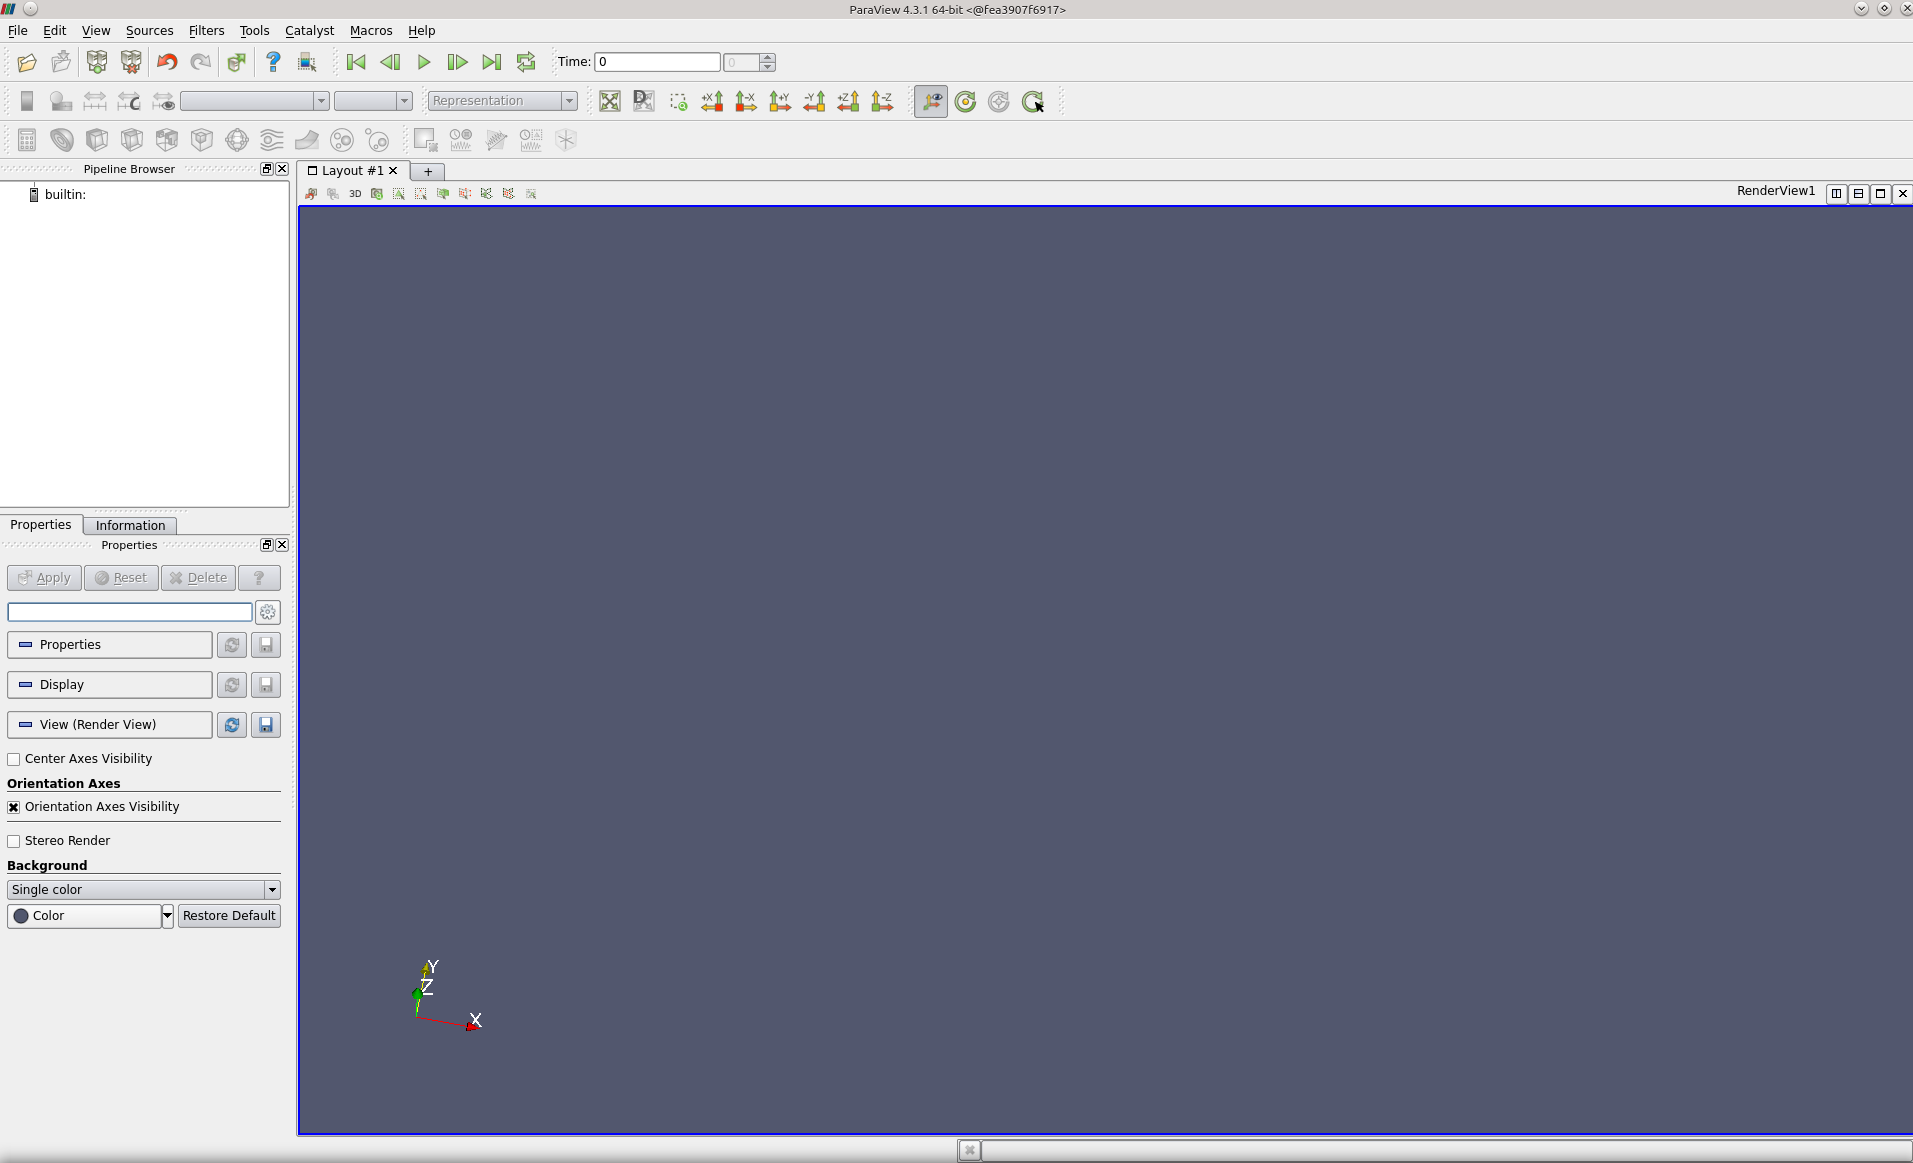
\includegraphics[width=\textwidth]{pictures/start_paraview.png}
    \caption{Start window of ParaView.}
    \label{ParaViewScreenshot}
\end{figure}

In order to analyze the numerical methods, change the following input parameters
\begin{itemize}
	\item stiffness in young modulus: 1000 up to 5000
	\item incompressibility in poisson ratio: 0.0 up to 0.49
\end{itemize}

The parameters can be changed by opening the XML-file in a suitable text editor, e.g.
\begin{lstlisting}[language=sh, breaklines=true]
$ geany /opt/msml/examples/LiverExample/liverLinear.msml.xml &
\end{lstlisting}


\section{Using the Python API}

This section describes how to create a running script for MSML in Python.
The absolute pathes are adapted to the pathes in the pre-built Docker container.

First open an editor (e.g. geany) and create a new file \emph{myScript.py}.
To run MSML from a python environment we need some imports as described in the following:
\begin{lstlisting}[language=Python]
import os
import sys
sys.path.insert(0, "/opt/msml/src") #to use msml imports
import msml.api.simulation_runner as api
\end{lstlisting}

Then you have to define the input file and the output directory:
\begin{lstlisting}[language=Python]
msml_infile = os.path.abspath("/opt/msml/examples/LiverExample/liverLinear.msml.xml")
msml_outdir = os.path.abspath("/tmp/MSMLResultsLiver/")
\end{lstlisting}

To start MSML the following code is necessary:
\begin{lstlisting}[language=Python]
myRunner = api.SimulationRunner(msml_infile, "sofa", msml_outdir)
myRunner.run()
\end{lstlisting}

Now your script is complete. Start the script with
\begin{lstlisting}[language=sh, breaklines=true]
$ python myScript.py
\end{lstlisting}
 
